\documentclass{article}
\usepackage{fullpage}
\usepackage{graphicx}
\usepackage[spanish]{babel}
\usepackage{amssymb}
\usepackage{amsmath}
\usepackage{cancel}
\usepackage{minted}
\usepackage[linesnumbered,ruled,lined]{algorithm2e}
\DontPrintSemicolon
\SetKwRepeat{Do}{do}{while}


%%%%% Comandos Personalizados %%%%%
\newcommand{\N}{\mathbb{N}}
\newcommand{\R}{\mathbb{R}}
\newcommand{\Q}{\mathbb{Q}}
\newcommand{\E}{\mathbb{E}}
\newcommand{\PP}{\mathbb{P}}
\newcommand{\la}{\leftarrow}
\newcommand{\ra}{\rightarrow}
\newcommand{\lra}{\leftrightarrow}
\newcommand{\Ra}{\Rightarrow}
\newcommand{\La}{\Leftarrow}
\newcommand{\LRa}{\Leftrightarrow}
\newcommand{\sub}{\subseteq}
\newcommand{\matro}{\mathcal{M}}

\newcommand{\twopartdef}[4]
{
	\left\{
		\begin{array}{ll}
			#1 &  \text{#2} \\
			#3 &  \text{#4}
		\end{array}
	\right.
}

%%%%%  Fin Comandos Personalizados %%%%%


     %%%%%%%%%% MODIFICAR %%%%%%%%%%
\newcommand{\alumnos}{Benja Sanchez, Victor Ruiz}
\newcommand{\departamento}{Departamento de Ingenieria Industrial y de Sistemas}
\newcommand{\ramo}{Optimización}
\newcommand{\sigla}{ICS1113}
\newcommand{\titulo}{Tarea 1}
\newcommand{\semestre}{01 }
\newcommand{\anio}{2023}
\newcommand{\med}{\frac{1}{2}}
\newcommand{\indep}{\mathcal{I}}
     %%%%%%%%%% FIN MODIFICAR %%%%%%%%%%



\renewcommand{\thesubsection}{\alph{subsection}}

\begin{document}

\thispagestyle{empty}

\begin{minipage}{2cm}
\vspace{-1.5cm}

\includegraphics[width=2cm]{logo.pdf}
\vspace{-1.4cm}
\end{minipage}
\begin{minipage}{\linewidth}
\textsc{\raggedright \footnotesize
Pontificia Universidad Católica de Chile \\
\departamento \\
\sigla - \ramo \\}
\end{minipage}

\begin{center}
\vspace{0.2cm}
{\huge\bf \titulo}\\
\vspace{1em}
{\large\bf{ Integrantes: \alumnos}}\\
\vspace{0.2cm}
\vspace{0.2cm}
\rule{\textwidth}{0.2mm}
\end{center}
\setcounter{secnumdepth}{0} % desactiva la numeración de las secciones

	
	\begin{flushleft}
		
		\section{Pregunta 1}
		a) \\
		$R_1$: $x_1 + 3x_2 \leq 9$ $\Rightarrow$ $x_2 \leq 3-\frac{x_1}{3} $ (Azul)\\
		$R_2$: $2x_1 + x_2 \leq 4$ $\Rightarrow$ $x_2 \leq 4-2x_1$ (Rojo)\\
		$R_3$: $x_1 + x_2 \leq 1$ $\Rightarrow$ $x_2 \geq 1-x_1 $ (Naranja)\\
		$R_4$: $x_1 \geq 0$ (Morado claro)\\
		$R_5$: $x_2 \geq 0$ (Verde)\\
		Región factible: (Morado)
		
		\vspace{0.5cm}

		\begin{figure}[ht]
			\centering
			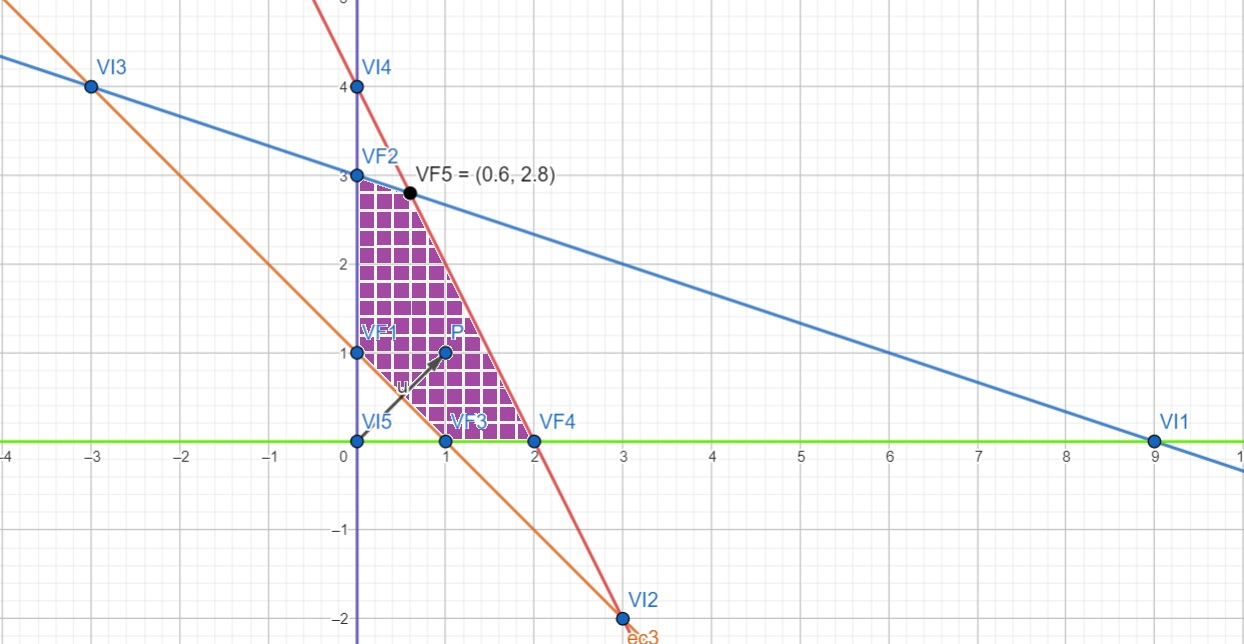
\includegraphics[width=1.1\textwidth]{grafico1.jpg}
			\caption{Gráfico pregunta 1}
			\label{fig:grafico}
		\end{figure}

		\newpage

		\begin{table}[ht]
			\centering
			\begin{minipage}{0.45\textwidth}
				\centering
				\begin{tabular}{|c|c|c|}
					\hline
					Vertice & Intersección & Coordenadas \\
					\hline
					$VF_1$ & $R_3$ y $R_4$ & $(0, 1)$ \\
					\hline
					$VF_2$ & $R_1$ y $R_4$ & $(0, 3)$\\
					\hline
					$VF_3$ & $R_3$ y $R_5$ & $(1, 0)$ \\
					\hline
					$VF_4$ & $R_2$ y $R_5$ & $(2, 0)$ \\
					\hline
					$VF_5$ & $R_2$ y $R_1$  & $(0.6, 2.8)$ \\
					\hline
				\end{tabular}
				\caption{Vertices Factibles}
				\label{tab:vertices_factibles}
			\end{minipage}
			\hfill
			\begin{minipage}{0.45\textwidth}
				\centering
				\begin{tabular}{|c|c|c|}
					\hline
					Vertice & Intersección & Coordenadas \\
					\hline
					${VI}_1$ & $R_1$ y $R_5$ & $(9, 0)$ \\
					\hline
					${VI}_2$ & $R_2$ y $R_3$ & $(3, -2)$\\
					\hline
					${VI}_3$ & $R_1$ y $R_3$  & $(-3, 4)$\\
					\hline
					${VI}_4$ & $R_4$ y $R_2$ & $(0, 4)$ \\
					\hline
					${VI}_5$ & $R_4$ y $R_5$  & $(0, 5)$ \\
					\hline
				\end{tabular}
				\caption{Vertices Infactibles}
				\label{tab:vertices_infactibles}
			\end{minipage}
		\end{table}
		\vspace{0,5cm}
		En el grafico y como se puede notar pór la forma de la función objetivo, el vertice fáctible que cumple con ser la solución optima es $VF_5$ dado que alcanza el valor máximo siendo $3.4$.\\
		
		
		\begin{table}[ht]
			\centering
			\begin{tabular}{|c|c|}
				\hline
				Restricción & Estado \\
				\hline
				$R_1$ & Activa \\
				$R_2$ & Activa \\
				$R_3$ & Inactiva \\
				$R_4$ & Inactiva \\
				$R_5$ & Inactiva \\
				\hline
			\end{tabular}
			\caption{Restricciones activas e inactivas en $VF_5$} 
			\label{tab:tabla_ejemplo}
		\end{table}
		\vspace{1cm}
		b) \\
		\vspace{0,5cm}
		\begin{center}
			\begin{align*}
				\text{P}) & \quad \min -x_1 - x_2 \\
				\text{s.a.} & \quad  R_1) \quad x_1 + 3x_2 \leq  9 \\
						   & \quad R_2) \quad 2x_1 + x_2 \leq  4 \\
						   & \quad R_3) \quad x_1 + x_2 \geq  1 \\
						   & \quad \quad x_1, x_2 \geq 0 \\
			\end{align*}
		\end{center}
		\begin{center}
			\begin{align*}
				\text{P} & \leftrightarrow \text{P} \\
			\end{align*}
		\end{center}

		\begin{center}
			\begin{align*}
				x_3) & \quad \text{Variable de holgura} \\
				x_4) & \quad \text{Variable de holgura} \\
				x_5) & \quad \text{Variable de exceso} \\
				\\
				\text{P}) & \quad \min -x_1 - x_2 \\
				\text{s.a.} & \quad  R_1) \quad x_1 + 3x_2 + x_3 = 9 \\
						   & \quad R_2) \quad 2x_1 + x_2 + x_4 = 4 \\
						   & \quad R_3) \quad x_1 + x_2 - x_5 = 1 \\
						   & \quad \quad x_1, x_2, x_3, x_4, x_5 \geq 0 \\
			\end{align*}
		\end{center}
		c) \\
		\vspace{0,5cm}
		
		\begin{center}
			\begin{align*}
				\text{P}) & \quad \min \quad x_6 + x_7 + x_8 \\
				\text{s.a.} & \quad  R_1) \quad x_1 + 3x_2 + x_3 + x_6 = 9 \\
						   & \quad R_2) \quad 2x_1 + x_2 + x_4 + x_7 = 4 \\
						   & \quad R_3) \quad x_1 + x_2 - x_5 + x_8 = 1 \\
						   & \quad \quad x_1, x_2, x_3, x_4, x_5, x_6, x_7, x_8 \geq 0 \\ 
			\end{align*}
		\end{center}
		
		Sea \( A \), \( \mathbf{b} \) y $x_B$:
		\begin{equation*}
			A =
			\left[
			\begin{array}{cccccccc}
			1 & 3 & 1 & 0 & 0 & 1 & 0  & 0  \\
			2 & 1 & 0 & 1 & 0 & 0 & 1 & 0 \\
			1 & 1 & 0 & 0 & -1 & 0 & 0 & 1  \\
			\end{array}
			\right], \quad
			\mathbf{b} =
			\left[
			\begin{array}{c}
			9 \\
			4 \\
			1 \\
			\end{array}
			\right], \quad
			C^\intercal =
			\left[
			\begin{array}{cccccccc}
			0 & 0 & 0 & 0 & 0 & 1 & 1 & 1 \\
			\end{array}
			\right].
		\end{equation*}
		
		Si $B = \{6,7,8\}$ entonces la matriz de coeficientes básicos, la matriz de coeficientes no básicos y la matriz de coeficientes básicos inversa son:
		\begin{equation*}
			\begin{array}{ccc}
				A_b = \begin{bmatrix}
					1 & 0 & 0 \\
					0 & 1 & 0 \\
					0 & 0 & 1 \\
				\end{bmatrix} &
				A_n = \begin{bmatrix}
					1 & 3 & 1 & 0 & 1  \\
					2 & 1 & 0 & 1 & 0 \\
					1 & 1 & 0 & 0 & 1 \\
				\end{bmatrix} &
				A_b^{-1} = \begin{bmatrix}
					1 & 0 & 0 \\
					0 & 1 & 0 \\
					0 & 0 & 1 \\
				\end{bmatrix}
			\end{array}
		\end{equation*}
		
		Luego $A_b^{-1}$b y $A_b^{-1}$$A_n$$X_n$ es:
		\begin{equation*}
			\begin{array}{cc}
				A_b^{-1}b = \begin{bmatrix}
					9 \\
					4 \\
					1 \\
				\end{bmatrix} &
				A_b^{-1}A_nX_n = \begin{bmatrix}
					1 & 3 & 1 & 0 & 1  \\
					2 & 1 & 0 & 1 & 0 \\
					1 & 1 & 0 & 0 & 1 \\
				\end{bmatrix}
				\begin{bmatrix}
					x_1 \\
					x_2 \\
					x_5 \\
				\end{bmatrix}
			\end{array}
		\end{equation*}

		\begin{figure}[ht]
			\centering
			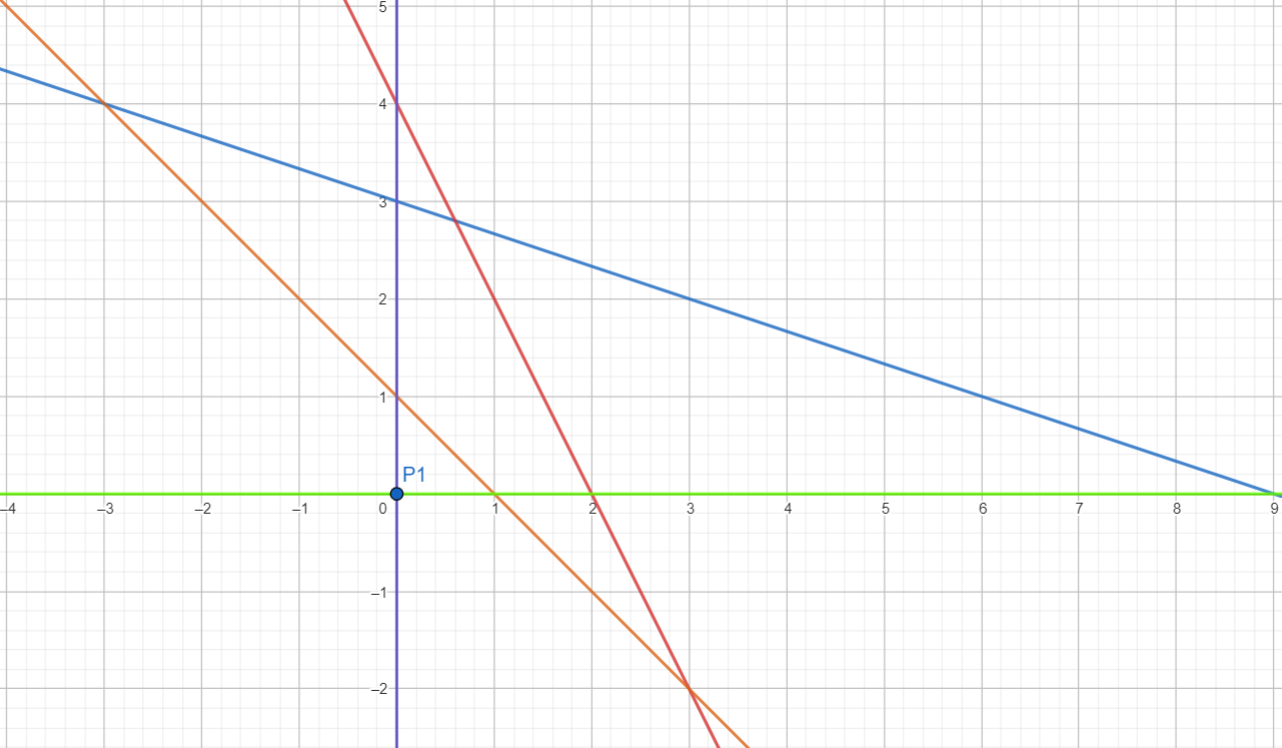
\includegraphics[width=0.5\textwidth]{grafico2.jpg}
			\caption{Fase 1 - Iteración 0}
			\label{fig:grafico}
		\end{figure}

		Con $C_n^\intercal$ y $C_b^\intercal$:
		\begin{equation*}
			\begin{array}{cc}
				C_n^\intercal = \begin{bmatrix}
					0 & 0 & 0\\
				\end{bmatrix} &
				C_b^\intercal = \begin{bmatrix}
					1 & 1 & 1  \\
				\end{bmatrix}
			\end{array}
		\end{equation*}

		Calculamos $C_b^\intercal$$A_b^{-1}$$A_n$:
		
		\begin{equation*}
			C_b^\intercal A_b^{-1}A_n = \begin{bmatrix}
				1 & 1 & 1 \\
			\end{bmatrix}
			\begin{bmatrix}
				1 & 3 & 1 & 0 & 1  \\
				2 & 1 & 0 & 1 & 0 \\
				1 & 1 & 0 & 0 & 1 \\	
			\end{bmatrix} = \begin{bmatrix}
				-4 & -5 & -1 & -1 & 1 \\
			\end{bmatrix}
		\end{equation*}

		Y entonces \(\bar{C}_n^\intercal\) = \(C_n^\intercal - C_b^\intercal A_b^{-1} A_n\) es:
		\begin{equation*}
			\bar{C}_n^\intercal = \begin{bmatrix}
				0 & 0 & 0\\
			\end{bmatrix} - \begin{bmatrix}
				-4 & -5 & -1 & -1 & 1 \\
			\end{bmatrix} = \begin{bmatrix}
				4 & 5 & 1 & 1 & -1 \\
			\end{bmatrix}
		\end{equation*}
		\vspace{0,5cm}
		
		Ya que hay costos reducidos negativos y buscamos incrementar $x_2$. \\


		Por lo tanto sale de la base $x_8$ y entra $x_2$ tal que la base nueva es $B = \{2,6,7\}$ y, $A_b$ y $A_n$\\


		\begin{equation*}
			\begin{array}{ccc}
				A_b = \begin{bmatrix}
					3 & 1 & 0 \\
					1 & 0 & 1 \\
					1 & 0 & 0 \\
				\end{bmatrix} &
				A_n = \begin{bmatrix}
					1 & 1 & 0 & 0 & 0\\
					2 & 0 & 1 & 0 & 0 \\
					1 & 0 & 0 & -1 & 1  \\
				\end{bmatrix} &
				A_b^{-1} = \begin{bmatrix}
					0 & 0 & 1 \\
					1 & 0 & -3 \\
					0 & 1 & -1 \\
				\end{bmatrix}
			\end{array}
		\end{equation*}

		Con $C_n^\intercal$ y $C_b^\intercal$:
		\begin{equation*}
			\begin{array}{cc}
				C_n^\intercal = \begin{bmatrix}
					0 & 0 & 0\\
				\end{bmatrix} &
				C_b^\intercal = \begin{bmatrix}
					1 & 1 & 1 \\
				\end{bmatrix}
			\end{array}
		\end{equation*}

		Y entonces \(\bar{C}_n^\intercal\) = \(C_n^\intercal - C_b^\intercal A_b^{-1} A_n\) es:
		\begin{align*}
			\bar{C}_n^\intercal = \begin{bmatrix}
				0 & 0 & 0 & 0 & 1\\
			\end{bmatrix} - \begin{bmatrix}
				0 & 1 & 1 \\
			\end{bmatrix} & \begin{bmatrix}
				0 & 0 & 1 \\
				1 & 0 & -3 \\
				0 & 1 & -1 \\
			\end{bmatrix} & \begin{bmatrix}
				1 & 1 & 0 & 0 & 0\\
				2 & 0 & 1 & 0 & 0 \\
				1 & 0 & 0 & -1 & 1  \\
			\end{bmatrix} = \begin{bmatrix}
				1 & -1 & -1 & -4 & 5\\
			\end{bmatrix}
		\end{align*}

		\begin{figure}[ht]
			\centering
			%\includegraphics[width=0.5\textwidth]{Fase_I_01.png}
			\caption{Fase 1 - Iteración 0}
			\label{fig:grafico}
		\end{figure}

		Por lo tanto x = (0,1,6,3,0,0) es la solución óptima, y como $y_1$ = 0 entonces se puede continuar con la Fase 2 con base factible $B = \{2,3,4\}$\\
		Por lo tanto sale de la base $x_6$ y entra $x_5$ tal que la base nueva es $B = \{2,5,7\}$ y, $A_b$ y $A_n$\\

		\vspace{0,5cm}

		
		d) \\
		\begin{center}
			\begin{align*}
				\text{P}) & \quad \min -x_1 - x_2 \\
				\text{s.a.} & \quad  R_1) \quad x_1 + 3x_2 + x_3 = 9 \\
						   & \quad R_2) \quad 2x_1 + x_2 + x_4 = 4 \\
						   & \quad R_3) \quad x_1 + x_2 - x_5 = 1 \\
						   & \quad R_4) \quad x_1\geq 0\\
						   & \quad R_5) \quad x_2 \geq 0 \\
						   & \quad R_6) \quad x_3 \geq 0 \\
						   & \quad R_7) \quad x_4 \geq 0 \\
						   & \quad R_8) \quad x_5 \geq 0 \\
			\end{align*}
		\end{center}

		Con A , $b$ y $C^\intercal$:
		\begin{equation*}
			A =
			\left[
			\begin{array}{ccccc}
			1 & 3 & 1 & 0 & 0 \\
			2 & 1 & 0 & 1 & 0 \\
			1 & 1 & 0 & 0 & -1  \\
			\end{array}
			\right], \quad
			\mathbf{b} =
			\left[
			\begin{array}{c}
			9 \\
			4 \\
			1 \\
			\end{array}
			\right], \quad
			C^\intercal =
			\left[
			\begin{array}{ccccc}
			-1 & -1 & 0 & 0 & 0\\
			\end{array}
			\right]
		\end{equation*}

		Si $B = \{2,3,4\}$ entonces la matriz de coeficientes básicos, la matriz de coeficientes no básicos y la matriz de coeficientes básicos inversa son:
		\begin{equation*}
			\begin{array}{ccc}
				A_b = \begin{bmatrix}
					3 & 1 & 0 \\
					1 & 0 & 1 \\
					1 & 0 & 0 \\
				\end{bmatrix} &
				A_n = \begin{bmatrix}
					1 & 0 \\
					2 & 0 \\
					1 & -1 \\
				\end{bmatrix} &
				A_b^{-1} = \begin{bmatrix}
					0 & 0 & 1\\
					1 & 0 & -3 \\
					0 & 1 & -1 \\
				\end{bmatrix}
			\end{array}
		\end{equation*}

		Luego $A_b^{-1}$b y $A_b^{-1}$$A_n$$X_n$ es:
		\begin{equation*}
			\begin{array}{cc}
				A_b^{-1}b = \begin{bmatrix}
					1 \\
					6 \\
					3 \\
				\end{bmatrix} &
				A_b^{-1}A_nX_n = \begin{bmatrix}
					1 & -1  \\
					-2 & 3 \\
					1 & 1 \\
				\end{bmatrix}
				\begin{bmatrix}
					x_1 \\
					x_5 \\
				\end{bmatrix}
			\end{array}
		\end{equation*}

		Con $C_n^\intercal$ y $C_b^\intercal$:
		\begin{equation*}
			\begin{array}{cc}
				C_n^\intercal = \begin{bmatrix}
					-1 & 0 \\
				\end{bmatrix} &
				C_b^\intercal = \begin{bmatrix}
					-1 & 0 & 0 \\
				\end{bmatrix}
			\end{array}
		\end{equation*}

		Calculamos $C_b^\intercal$$A_b^{-1}$$A_n$:
		
		\begin{equation*}
			C_b^\intercal A_b^{-1}A_n = \begin{bmatrix}
				-1 & 0 & 0 \\
			\end{bmatrix}
			\begin{bmatrix}
				1 & -1 &\\
				-2 & 3 & \\
				1 & 1 & \\
			\end{bmatrix} = \begin{bmatrix}
				-1 & 1\\
			\end{bmatrix}
		\end{equation*}

		Y entonces \(\bar{C}_n^\intercal\) = \(C_n^\intercal - C_b^\intercal A_b^{-1} A_n\) es:
		\begin{equation*}
			\bar{C}_n^\intercal = \begin{bmatrix}
				-1 & 0 \\
			\end{bmatrix} - \begin{bmatrix}
				-1 & 1\\
			\end{bmatrix} = \begin{bmatrix}
				0 & -1\\
			\end{bmatrix}
		\end{equation*}

		\begin{figure}[ht]
			\centering
			%\includegraphics[width=0.5\textwidth]{Fase_I_01.png}
			\caption{Fase 2 - Iteración 0}
			\label{fig:grafico}
		\end{figure}

		Ya que hay costos reducidos negativos fijamos $x_1$ en 0 y buscamos incrementar $x_5$. Para eso calculamos taza de razón mínima de $x_5$\\

		\begin{equation*}
			\begin{array}{cc}
				\min \left\{ \frac{6}{3}, \frac{3}{1} \right\} = 2 
			\end{array}
		\end{equation*}

		Por lo tanto sale de la base $x_3$ y entra $x_5$ tal que la base nueva es $B = \{2,4,5\}$ y, $A_b$ y $A_n$\\

		\begin{equation*}
			\begin{array}{ccc}
				A_b = \begin{bmatrix}
					3 & 0 & 0 \\
					1 & 1 & 0\\
					1 & 0 & -1 \\
				\end{bmatrix} &
				A_n = \begin{bmatrix}
					1 & 1\\
					2 & 0\\
					1 & 0 \\
				\end{bmatrix} &
				A_b^{-1} = \begin{bmatrix}
					1/3 & 0  & 0 \\
					-1/3 & 1  & 0 \\
					1/3 & 0  & -1 \\
				\end{bmatrix}
			\end{array}
		\end{equation*}

		Luego $A_b^{-1}$b y $A_b^{-1}$$A_n$$X_n$ es:
		\begin{equation*}
			\begin{array}{cc}
				A_b^{-1}b = \begin{bmatrix}
					3  \\
					1 \\
					2 \\
				\end{bmatrix} &
				A_b^{-1}A_nX_n = \begin{bmatrix}
					1/3 & 1/3  \\
					5/3 & -1/3 \\
					-2/3 & 1/3 \\
				\end{bmatrix}
				\begin{bmatrix}
					x_1 \\
					x_3 \\
				\end{bmatrix}
			\end{array}
		\end{equation*}

		Con $C_n^\intercal$ y $C_b^\intercal$:
		\begin{equation*}
			\begin{array}{cc}
				C_n^\intercal = \begin{bmatrix}
					-1 & 0 \\
				\end{bmatrix} &
				C_b^\intercal = \begin{bmatrix}
					-1 & 0 & 0 \\
				\end{bmatrix}
			\end{array}
		\end{equation*}

		Calculamos $C_b^\intercal$$A_b^{-1}$$A_n$:
		
		\begin{equation*}
			C_b^\intercal A_b^{-1}A_n = \begin{bmatrix}
				-1 & 0 & 0 \\
			\end{bmatrix}
			\begin{bmatrix}
				1/3 & 1/3  \\
				5/3 & -1/3 \\
				-2/3 & 1/3 \\
			\end{bmatrix} = \begin{bmatrix}
				-1/3 & -1/3\\
			\end{bmatrix}
		\end{equation*}

		Y entonces \(\bar{C}_n^\intercal\) = \(C_n^\intercal - C_b^\intercal A_b^{-1} A_n\) es:
		\begin{equation*}
			\bar{C}_n^\intercal = \begin{bmatrix}
				-1 & 0 \\
			\end{bmatrix} - \begin{bmatrix}
				-1/3 & 1/3\\
			\end{bmatrix} = \begin{bmatrix}
				-2/3 & 1/3\\
			\end{bmatrix}
		\end{equation*}

		\begin{figure}[ht]
			\centering
			%\includegraphics[width=0.4\textwidth]{Fase_II_03.png}
			\caption{Fase 2 - Iteración 1}
			\label{fig:grafico}
		\end{figure}

		Ya que hay costos reducidos negativos fijamos $x_3$ en 0 y buscamos incrementar $x_1$. Para eso calculamos taza de razón mínima de $x_1$\\


		
		\begin{equation*}
			\begin{array}{cc}
				\min \left\{ 9, \frac{3}{5} \right\} = 2 
			\end{array}
		\end{equation*}

		Por lo tanto sale de la base $x_4$ y entra $x_1$ tal que la base nueva es $B = \{1,2,5\}$ y, $A_b$ y $A_n$\\

		\begin{equation*}
			\begin{array}{ccc}
				A_b = \begin{bmatrix}
					1 & 3 & 0 \\
					2 & 1 & 0\\
					1 & 1 & -1 \\
				\end{bmatrix} &
				A_n = \begin{bmatrix}
					1 & 0 \\
					0 & 1 \\
					0 & 0 \\
				\end{bmatrix} &
				A_b^{-1} = \begin{bmatrix}
					-1/5 & 3/5 & 0\\
					2/5 & -1/5 & 0 \\
					1/5 & 2/5 & -1 \\
				\end{bmatrix}
			\end{array}
		\end{equation*}

		Luego $A_b^{-1}$b y $A_b^{-1}$$A_n$$X_n$ es:
		\begin{equation*}
			\begin{array}{cc}
				A_b^{-1}b = \begin{bmatrix}
					3/5\\
					14/5 \\
					12/5 \\
				\end{bmatrix} &
				A_b^{-1}A_nX_n = \begin{bmatrix}
					-1/5 & 3/5  \\
					2/5 & -1/5 \\
					1/5 & 2/5  \\
				\end{bmatrix}
				\begin{bmatrix}
					x_3 \\
					x_4 \\
				\end{bmatrix}
			\end{array}
		\end{equation*}

		Con $C_n^\intercal$ y $C_b^\intercal$:
		\begin{equation*}
			\begin{array}{cc}
				C_n^\intercal = \begin{bmatrix}
					0 & 0 \\
				\end{bmatrix} &
				C_b^\intercal = \begin{bmatrix}
					-1 & -1 & 0 \\
				\end{bmatrix}
			\end{array}
		\end{equation*}

		Calculamos $C_b^\intercal$$A_b^{-1}$$A_n$:
		\begin{equation*}
			C_b^\intercal A_b^{-1}A_n = \begin{bmatrix}
				-1 & -1 & 0 \\
			\end{bmatrix}
			\begin{bmatrix}
				-1/5 & 3/5  \\
				2/5 & -1/5 \\
				1/5 & 2/5  \\
			\end{bmatrix} = \begin{bmatrix}
				-1/5 & -2/5\\
			\end{bmatrix}
		\end{equation*}

		Y entonces \(\bar{C}_n^\intercal\) = \(C_n^\intercal - C_b^\intercal A_b^{-1} A_n\) es:
		\begin{equation*}
			\bar{C}_n^\intercal = \begin{bmatrix}
				0 & 0 \\
			\end{bmatrix} - \begin{bmatrix}
				-1/5 & -2/5\\
			\end{bmatrix} = \begin{bmatrix}
				1/5 & 2/5\\
			\end{bmatrix}
		\end{equation*}

		\begin{figure}[ht]
			\centering
			%\includegraphics[width=0.4\textwidth]{Fase_II_opti.png}
			\caption{Fase 2 - Iteración 2}
			\label{fig:grafico}
		\end{figure}

		Ya que no hay costos reducidos negativos, la solución óptima es x = (3/5,14/5,0,0,12/5) y el valor óptimo es -17/5.\\
		\vspace{12cm}

		e) Por alguna razón, se generó cierta variación $\delta$ en el recurso (4) de la restricción $R_2$. Indique mediante un argumento gráfico entre qué valores puede estar $\delta$ para mantener la configuración de base óptima actual sin que haya degenerancia. Indique los valores que debe tomar delta para que haya degenerancia en la base óptima actual.\\
		\vspace{1cm}

		Primero notamos que la región factible sin la restricción $R_2$ es la siguiente:\\

		\begin{figure}[ht]
			\centering
			%\includegraphics[width=0.8\textwidth]{Región_Factible.png}
			\caption{Región factible sin $R_2$}
			\label{fig:grafico}
		\end{figure}

		Luego notamos que al variar $\delta$ la restricción $R_2$ se desplaza hacia los lados siempre intersectando con $R_1$ y este punto se econtrará en la región factible siempre y cuando $\delta$ $\in (-1,14)$.\\ 

		\begin{figure}[ht]
			\centering
			%\includegraphics[width=0.8\textwidth]{Región_Factible_1.png}
			\caption{Región factible $\gamma = -1$}
			\label{fig:grafico}
		\end{figure}

		\begin{figure}[ht]
			\centering
			%\includegraphics[width=0.8\textwidth]{Región_Factible_2.png}
			\caption{Región factible $\gamma = 14$}
			\label{fig:grafico}
		\end{figure}

		\vspace{4cm}

		Sin embargo como nuestra Base $B = \{1,2,5\}$, si $\delta$ $= \{1,14\}$ entonces la solución es degenerada. Por lo tanto para mantener la base óptima y que no haya degerancia $\delta \in (-1,14)$ \\

		\vspace{1cm}



		2. Sea $P = \{x \in \mathbb{R}^n : Ax = b, x \geq 0\}$ un poliedro en forma estándar no vacío definido por $m$ restricciones $a_i^T x = b_i$ para $i = 1, \ldots, m$ tales que la matriz $A$ tiene filas linealmente dependientes.\\
		\vspace{0,5cm}

		a) Explique por qué, sin pérdida de generalidad, podemos suponer que existen escalares $\lambda_1, \ldots, \lambda_{m-1} \in \mathbb{R}$ tales que $\sum_{i=1}^{m-1} \lambda_i a_i = a_m$.\\
		\vspace{0,5cm}

		b) Explique por qué podemos remover la restricción $a_m^T x = b_m$ sin que $P$ se vea alterado.\\
		\vspace{0,5cm}

		c) ¿Cómo se relaciona lo anterior con el supuesto de filas linealmente independientes en el método simplex?\\

		\subsection{Conjuntos}
		\begin{itemize}
			\item P) max    $x_1 + x_2$

		\end{itemize}

		\subsection{Parámetros}
		\begin{itemize}
			\item $C_{bn}$, costo de viajar desde $b$ hasta $n$.
			\item $CL_b$, tarifa de pasar la noche en el estacionamiento $b$.
			\item $D_{nt}$, demanda de agua en el punto $n$ el día $t$.
		\end{itemize}

		\subsection{Variables de decisión} 
		\begin{itemize}
			\item $x_{ktbn}$, una variable binaria que indica si el cam\'ion $k$ en el d\'ia $t$ viaja desde $b$ hasta $n$ ($x_{ktbn} = 1$) o no ($x_{ktbn} = 0$).
			\item $x_{ktnb}$, una variable binaria que indica si el cam\'ion $k$ en el d\'ia $t$ viaja desde $n$ hasta $b$ ($x_{ktnb} = 1$) o no ($x_{ktnb} = 0$).
			\item $y_{kbt}$, una variable binaria que indica si el cam\'ion $k$ pasa la noche en el estacionamiento $b$  en el dia $t$ ($y_{kbt} = 1$) o no ($y_{kbt} = 0$).
			\item $z_{kt}$, cantidad de agua transportada por el cami\'on $k$ en el d\'ia $t$.
		\end{itemize}

		\subsection{Función Objetivo}
		\begin{quote}
			\begin{center}
				Minimizar $\sum\limits_{n \in N}\sum\limits_{b \in \Theta}\sum\limits_{k \in \Gamma}\sum\limits_{t \in T} C_{bn} \cdot x_{ktbn} + C_{nb} \cdot x_{ktbnb} + CL_b \cdot y_{kbt}$
			\end{center}
		\end{quote}

		\subsection{Restricciones}
		\begin{itemize}
			\item $\sum\limits_{k \in \Gamma} z_{kt} = D_{nt} \hspace{1em} \forall \hspace{1mm} t \hspace{0mm} \in T, \hspace{1mm} \forall \hspace{1mm} n \in N $  (restricci\'on de satisfacci\'on de demanda diaria)
			\item $z_{kt} \leq W$ (Restricción de capacidad de transporte)
			\item $\sum\limits_{n \in N} x_{ktbn} \leq 1$ (restricción de cantidad de viajes por día)
			\item $\sum\limits_{b \in \Theta} y_{kbt} = 1$ (Restricción de capacidad de transporte)
			\item $\sum\limits_{n \in N} x_{ktbn} = 1$ (Restricción de capacidad de transporte)
		\end{itemize}

		\subsection{Naturaleza de las variables}
		\begin{itemize}
			\item $C_{bn},\hspace{1mm} CL_{b},\hspace{1mm} D_{nt},\hspace{1mm} z_{kt} \geq 0$ son variables binarias
			\item $z_{ktbn},\hspace{1mm} x_{ktnb},\hspace{1mm} y_{ktb} \in \{0,1\}$.
		\end{itemize}
		
		\section{Problema 2}
		La empresa Rayos tiene el monopolio de generación y transmisión de energía eléctrica en el país Demo. Rayos quiere minimizar sus costos, satisfaciendo la demanda en un día típico de 24 horas. A lo largo y ancho del país, la empresa tiene instalado un conjunto $N$ de plantas generadoras. Además, existe un conjunto $M$ de nodos de consumo eléctrico en el país. Para cada hora $h \in H = \{1, ..., 24\}$, existe una demanda de $D_{m,h}$ MWh que debe llegar al nodo de consumo de índice $m \in M$, después de restar las pérdidas en los cables. Cada generadora $n \in N$ decide cuánta energía en MWh envía de manera constante a cada nodo durante cada hora $h \in H$, sin superar su capacidad máxima de producción por hora que es $C_{Nn,h}$. Todas las generadoras están apagadas inicialmente, sin poder producir. Sin embargo, si se decide encender la generadora $n \in N$ en la hora $h \in H$, entonces desde esa hora se podrá producir hasta el final del día costando $c_{n,h}$ pesos dicha acción. Existe un conjunto $\Phi$ que contiene todos los pares $(n, m)$ tales que existe una conexión única por cable entre la generadora $n \in N$ y el nodo $m \in M$. Para cada conexión, existe una pérdida de la energía enviada por concepto de resistencia normal y resistencia no ohmica en los cables. Esta pérdida de energía es proporcional a la energía enviada, según un coeficiente de pérdida $R_{n,m}$, entre la generadora $n \in N$ y el nodo de consumo $m \in M$. Además, el parámetro $G_{n,m}$ (medido en $\frac{1}{\text{MWh}}$) representa un factor que debe multiplicarse por el cuadrado de la energía enviada cada hora para obtener la energía perdida en el cable por su comportamiento no ohmico. Además, esa conexión solo puede transmitir un máximo de $C_{Ln,m}$ MWh cada hora. Si $(n, m) \notin \Phi$, entonces $R_{n,m}$, $G_{n,m}$ y $C_{Ln,m}$ deben ser ignorados. El costo medio variable de generar $L$ unidades de energía (MWh) está determinado en cada planta $n \in N$ y en cada hora $h \in H$ por una función afin decreciente: $CM_{eV}(L) = a_{n,h} - b_{n,h} \cdot L$. Se debe considerar que la unidad de medida de $a_{n,h}$ es pesos/MWh, y que la de $b_{n,h}$ es pesos por cada unidad de $pesos/(MWh)^2h$. El costo de producir, en una hora de generación, se obtiene multiplicando lo producido por el costo medio variable de producir esa cantidad.\\
		\vspace{5mm}
		Formule un modelo de optimización no lineal que ayude a la empresa Rayos a minimizar sus costos en total satisfaciendo la demanda de todos los nodos de consumo del país. Escriba claramente las variables de decisión, restricciones y función objetivo del modelo.\\
		
			

		\subsection{Conjuntos}
		\begin{itemize}
			\item $n \in \{1, \ldots, N\}$, número de planta generadora.
			\item $m \in \{1, \ldots, M\}$, número de nodos de consumo electrico.
			\item $h \in \{1, \ldots, H\}$, número de horas del día.
		\end{itemize}
		
		\subsection{Parámetros}
		\begin{itemize}
			\item $D_{mh}$, demanda que debe llegar al nodo $m$ en la hora $h$.
			\item $CN_{nh}$, capacidad máxima de produción de la planta $n$ en la hora $h$.
			\item $c_{nh}$, coste de producción de la planta $n$ por $h$ horas. 
			\item $R_{nm}$, coeficiente de perdida de energia entre la planta $n$ y el nodo $m$.
			\item $G_{nm}$, parametro para calcular la energía perdida entre $n$ y $m$
			\item $CL_{nm}$, capacidad máxima de transmision entre la planta $n$ y el nodo $m$. 
			\item $CMeV(L)$, función afín decreciente que define el costo medio variable de generar L unidades de energía. 
			\item $a_{nh}$, coste de producción de la planta $n$ por $h$ horas. 
			\item $b_{nh}$, coste de producción de la planta $n$ por $h$ horas. 
		\end{itemize}
		\subsection{Variables de decisión} 
		\begin{itemize}
			\item $E_{nh}$, energía enviada a los nodos $n$ en la hora $h$.
			\item $x_{nh}$, variable binaria que indica si la planta $n$ en la hora $h$ está encendida ($X_{nh} = 1$) o no ($X_{nh} = 1$).
			\item $E_{base}$, energía básica o mínima que se debe enviar a un nodo
			\item $y_{nh}$, variable binaria que indica si la planta $n$ fué encendida en la hora $h$ ($X_{nh} = 1$) o no ($X_{nh} = 1$).
		\end{itemize}
		\subsection{Función Objetivo}
		\begin{quote}
			\begin{center}
				Min $\sum\limits_{h \in H}\sum\limits_{n \in N} C_{nh} \cdot y_{nh} + (a_{nh} - b_{nh} \cdot E_{nh})\cdot E_{nh}$
			\end{center}
		\end{quote}
		\subsection{Restricciones}
		\begin{itemize}
			\item $\sum\limits_{n \in N} (E_{nh} - E{nh} \cdot R_{nm} - E_{nm}^2 \cdot G_{nm}) = D_{mh} \hspace{1em} \forall \hspace{1mm} (n,m) \in \Phi \hspace{1mm} \forall \hspace{1mm} n \in  H$ (Restricción satisfacción de demanda)
			\item $E_{nh} \leq CN{nh} \hspace{1em} \forall \hspace{1mm} n \in N \hspace{1mm} \forall \hspace{1mm} h \in H$ (Restricción de producción de energía)
			\item $E_{nh} \leq CL{nh} \hspace{1em} \forall \hspace{1mm} (n,m) \in \Phi \hspace{1mm} \forall \hspace{1mm} h \in H$ (Restricción de transmision de energía)
			\item $\sum\limits_{n \in N} E_{nh} = D{mh} \hspace{1em} \forall \hspace{1mm} (n,m) \notin \Phi \hspace{1mm} \forall \hspace{1mm} h \in H$ (Cables sin restrición de capacidad)
			\item $E_{nh} \geq x_{nh} \cdot E_{base} \hspace{1em} \forall \hspace{1mm} n \in N \hspace{1mm} \forall \hspace{1mm} h \in H$ (Restriccion de energía mínima)
			\item $x_{nh} \leq x_{n,h+1} \hspace{1em} \forall \hspace{1mm} n \in N \hspace{1mm} \forall \hspace{1mm} h \in [0,24)$ (Restricción de que una vez prendida no se puede apagar)
		\end{itemize}
		\subsection{Naturaleza de las variables}
		\begin{itemize}
			\item $D_{nm},\hspace{1mm} E_{nm},\hspace{1mm} CN_{nh},\hspace{1mm} C_{nh},\hspace{1mm} CL_{nm},\hspace{1mm} R_{nm},\hspace{1mm} G_{nm},\hspace{1mm} E_{base} \geq 0 \hspace{1em} \forall \hspace{1mm} n \in N \hspace{1mm} \forall \hspace{1mm} h \in H \hspace{1mm} \forall \hspace{1mm} m \in M $
			\item $x_{nm},\hspace{1mm} y_{nh} \in \{0,1\} \hspace{1em}\forall \hspace{1mm} n \in N \hspace{1mm} \forall \hspace{1mm} h \in H \hspace{1mm} \forall \hspace{1mm} m \in M$
		\end{itemize}
	\end{flushleft}	
\end{document}	
